% Gemini theme
% https://github.com/anishathalye/gemini

\documentclass[final]{beamer}

% ====================
% Packages
% ====================

\usepackage[T1]{fontenc}
\usepackage[size=custom,width=120,height=72,scale=1.0]{beamerposter}
\usetheme{gemini}
\usecolortheme{gemini}
\usepackage{graphicx}
\usepackage{booktabs}
\usepackage{pgfplots}
\usepackage{subfig}
\usepackage{wrapfig}

\pgfplotsset{compat=1.17}

\usepackage{lmodern}

\makeatletter
\let\@@magyar@captionfix\relax
\makeatother

\makeatletter
\DeclareRobustCommand{\rvdots}{%
  \vbox{
    \baselineskip8\p@\lineskiplimit\z@
    \kern-\p@
    \hbox{.}\hbox{.}\hbox{.}
  }}
\makeatother

\newcommand{\bigCI}{\mathrel{\text{\scalebox{1.07}{$\perp\mkern-10mu\perp$}}}}

\definecolor{lgrey}{HTML}{CDCDCD}
\definecolor{white}{HTML}{FFFFFF}
\definecolor{black}{HTML}{000000}
\definecolor{nclBlue}{HTML}{003A65}
\definecolor{nclBlue2}{HTML}{759FBC}
\definecolor{nclRed}{HTML}{D91A35}
\definecolor{nclRedShade}{HTML}{EA8290}
\definecolor{nclBlend}{HTML}{6D2A4D}

% ====================
% Lengths
% ====================

% If you have N columns, choose \sepwidth and \colwidth such that
% (N+1)*\sepwidth + N*\colwidth = \paperwidth
\newlength{\sepwidth}
\newlength{\colwidth}
\setlength{\sepwidth}{0.025\paperwidth}
\setlength{\colwidth}{0.3\paperwidth}

\newcommand{\separatorcolumn}{\begin{column}{\sepwidth}\end{column}}
\newcommand{\halfseparatorcolumn}{\begin{column}{0.01\paperwidth}\end{column}}

\graphicspath{{images/}}

% ====================
% Title
% ====================

\title{Identification and impact assessment of recurring traffic bottlenecks using ANPR cameras}

\author{Pedro Pinto da Silva \inst{1} \and Matthew Forshaw \inst{1} \and Phil Blythe \inst{2} \and Stephen McGough \inst{1}}

\institute[shortinst]{\inst{1} School of Computing, Newcastle University \samelineand \inst{2} School of Engineering, Newcastle University}

% ====================
% Body
% ====================

\begin{document}

\begin{frame}[t]
\begin{columns}[t]
\separatorcolumn

\begin{column}{\colwidth}

  \begin{block}{Recurring traffic bottlenecks}

    \heading{What are recurring bottlenecks?}

        Bottlenecks are one of the main sources of traffic \emph{congestion}.
        In particular, recurring bottlenecks are characterised by their
        predictability: when and where they occur, and their impact on traffic
        flow. Recurring bottlenecks, as opposed to congestion caused by sporadic
        incidents, are of special interest to traffic managers because they are
        associated with operational deficiencies often eligible for remediation.
        The identification and ranking of bottlenecks, in terms of experienced
        delay and variability, is therefore crucial for the prioritisation of
        interventions aiming to mitigate bottleneck-induced congestion
        \cite{spiller2017}.

        \begin{figure}
          \subfloat{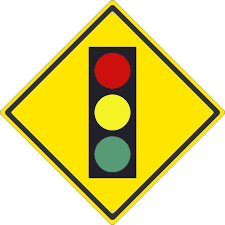
\includegraphics[width=0.125\linewidth]{traffic_light.png}}\hfill
          \subfloat{
\includegraphics[width=0.125\linewidth]{roundabout.png}}\hfill
          \subfloat{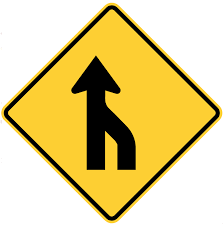
\includegraphics[width=0.125\linewidth]{merge_left.png}}\hfill
          \subfloat{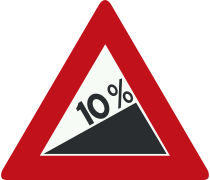
\includegraphics[width=0.125\linewidth]{grades.png}}\hfill
          \subfloat{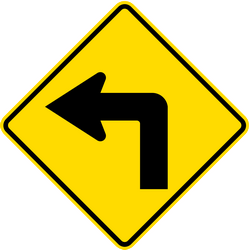
\includegraphics[width=0.125\linewidth]{sharp_curve.png}}
          \caption{Example of several operational elements that may cause
                   recurring bottlenecks.}
          \label{fig:bottleneck_causes}
        \end{figure}


    \heading{Characteristics of a bottleneck}

    \begin{wrapfigure}{r}{0.55\linewidth}
      \vspace{-0.5cm}
      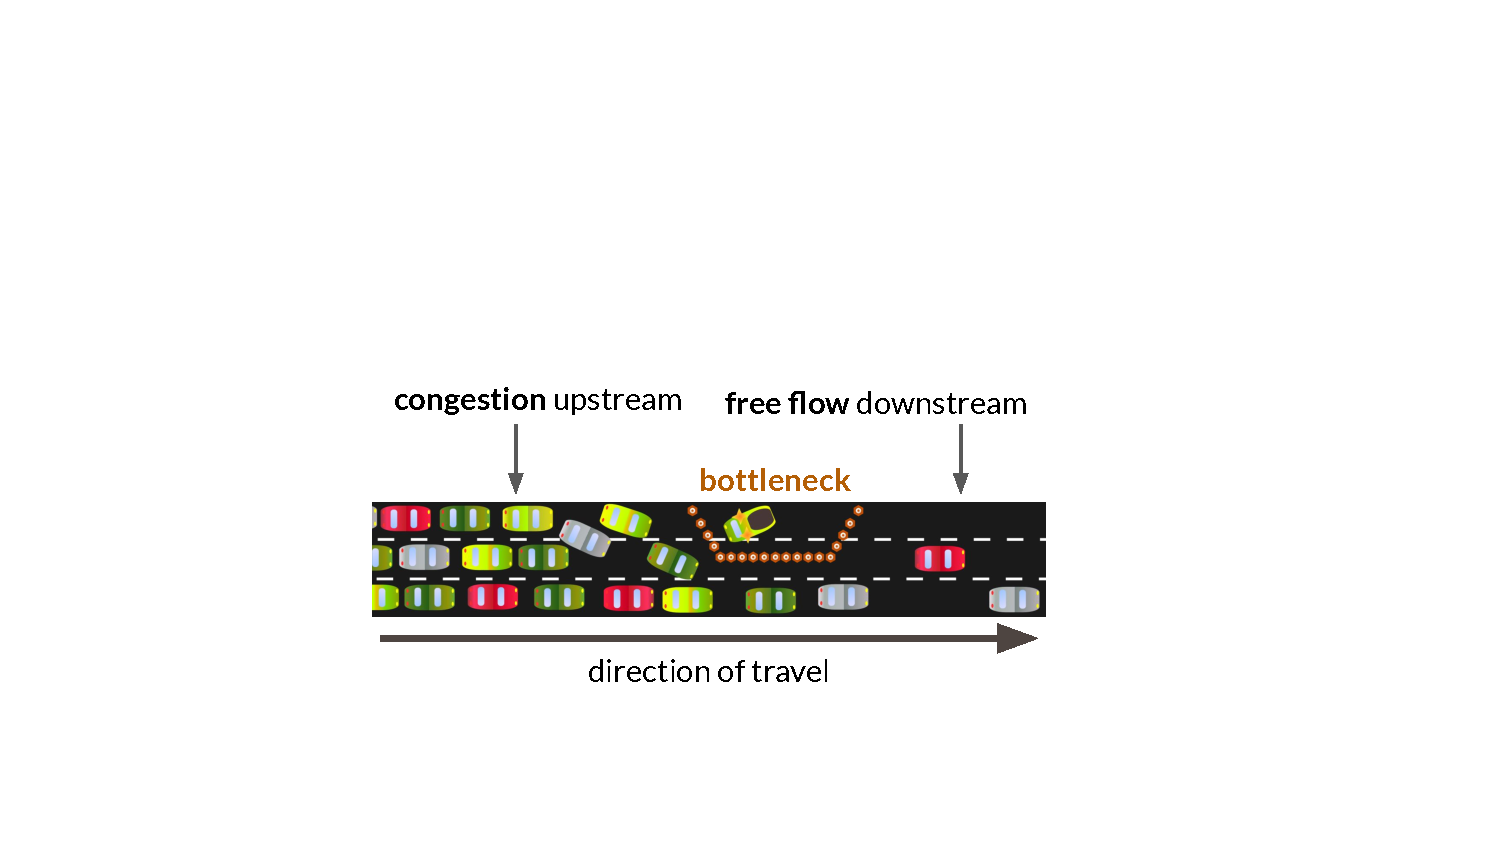
\includegraphics[width=0.95\linewidth]{bottleneck.pdf}
      \caption{Conceptual schematic of a bottleneck.}
      \label{fig:}
    \end{wrapfigure}

    An active bottleneck has four distinctive features:
    (i) congestion upstream of the bottleneck,
    characterised by slower speeds and longer travel times, (ii) free flow
    conditions downstream of the location, (iii) operation under
    considerable demand and (iv) existence of a specific point where traffic
    breaksdows and a queue starts to form upstream, in other words, a clear
    indication that congestion is localised rather than systemic.

    \heading{Knowledge gap}

    Research on bottleneck identification and their impact has been done
    almost exclusively on \emph{highways}. Some reasons for this are:

    \begin{itemize}
      \item Highways carry large volumes of traffic and bottlenecks can
            incur severe economic and social costs.
      \item Highways approximate idealised roads, with few entry and exit
            points, which makes the measurement of traffic flow easier and less
            costly.
    \end{itemize}

    Local traffic authorities. By extending the body of bottleneck research to
    a larger variety of road types and network topologies

    This will, in turn, strengthen the proposal for funds  that are put forward by
    local traffic authorities


  \end{block}

  \begin{alertblock}{Opportunity: Automatic Number Plate Recognition (ANPR) cmeras}

    ANPR cameras distinguish themselves from traditional traffic sensors, such
    as loop detectors and CCTV cameras, by their ability to identify and record
    the number plate of vehicles. Local traffic authorities have started to
    employ large groups of ANPR cameras in corridors across urban centres in
    order to actively monitor and report traffic conditions, particularly travel
    time, to drivers in real-time.

    Since we can identify individual vehicles we are , with the appropriate
    data security and privacy measures in place,

    They offer new insights into individual and aggregate travel patterns of
    vehicles within cities and have the potential to transform traffic
    monitoring and control.

    \textbf{Challenges:} Duplicates, bad number plates, low confidence
    observations, invalid observations, trip identification, network graph
    from OpenStreetMap data, mapping cameras to edges in the network graph,
     shortest path assumption, calculating distances, anonymisation, ...


  \end{alertblock}

\end{column}

\separatorcolumn

\begin{column}{\colwidth}

  \begin{block}{Bottleneck identification }

    \heading{Motivating example}

    \begin{wrapfigure}{r}{0.60\linewidth}
      \centering
      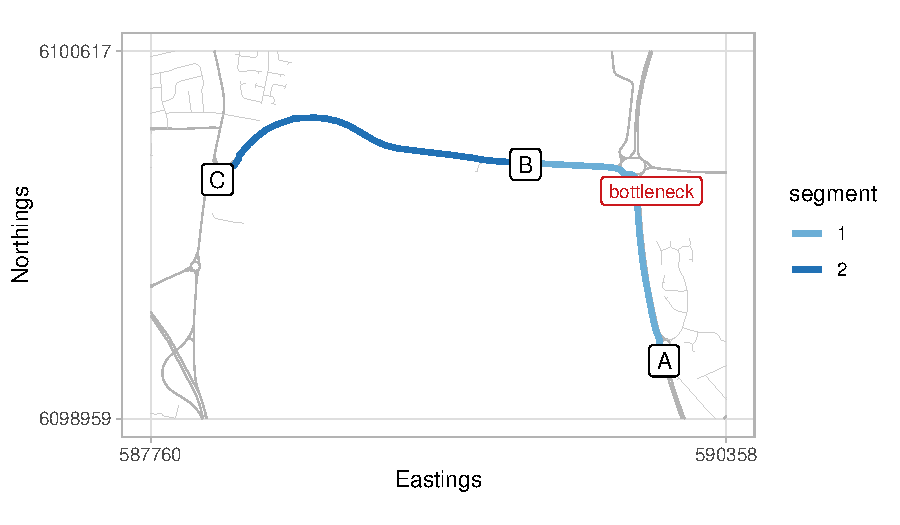
\includegraphics[width=0.95\linewidth]{MOTIVATING-EXAMPLE-map.pdf}
      \caption{The A1056 Killingworthway roundabout, an infamous bottleneck,
               and North-Westbound corridor monitored by 3 ANPR cameras.}
               \label{fig:motivating_example_map}
    \end{wrapfigure}

    An instance of the bottleneck identification problem is depicted in
    Figure \ref{fig:motivating_example_map}. The A1504 Killingworthway
    roundabout is a well known bottleneck which slows down vehicles that
    travelling North (location 'A') and then Westbound (location 'C' via 'B').
    The effect can be observed in Figure \ref{fig:motivating_example_1dayplots},
    which depicts the count (left) and mean speed (right) of vehicles driving
    through each segment of the corridor, on 5-minute time windows. We can
    clearly see that vehicles move generally slower on the first segment,
    particularly during the evening peak-hour, a behaviour suggestive of
    bottleneck activation.

    \begin{figure}
      \centering
      \subfloat{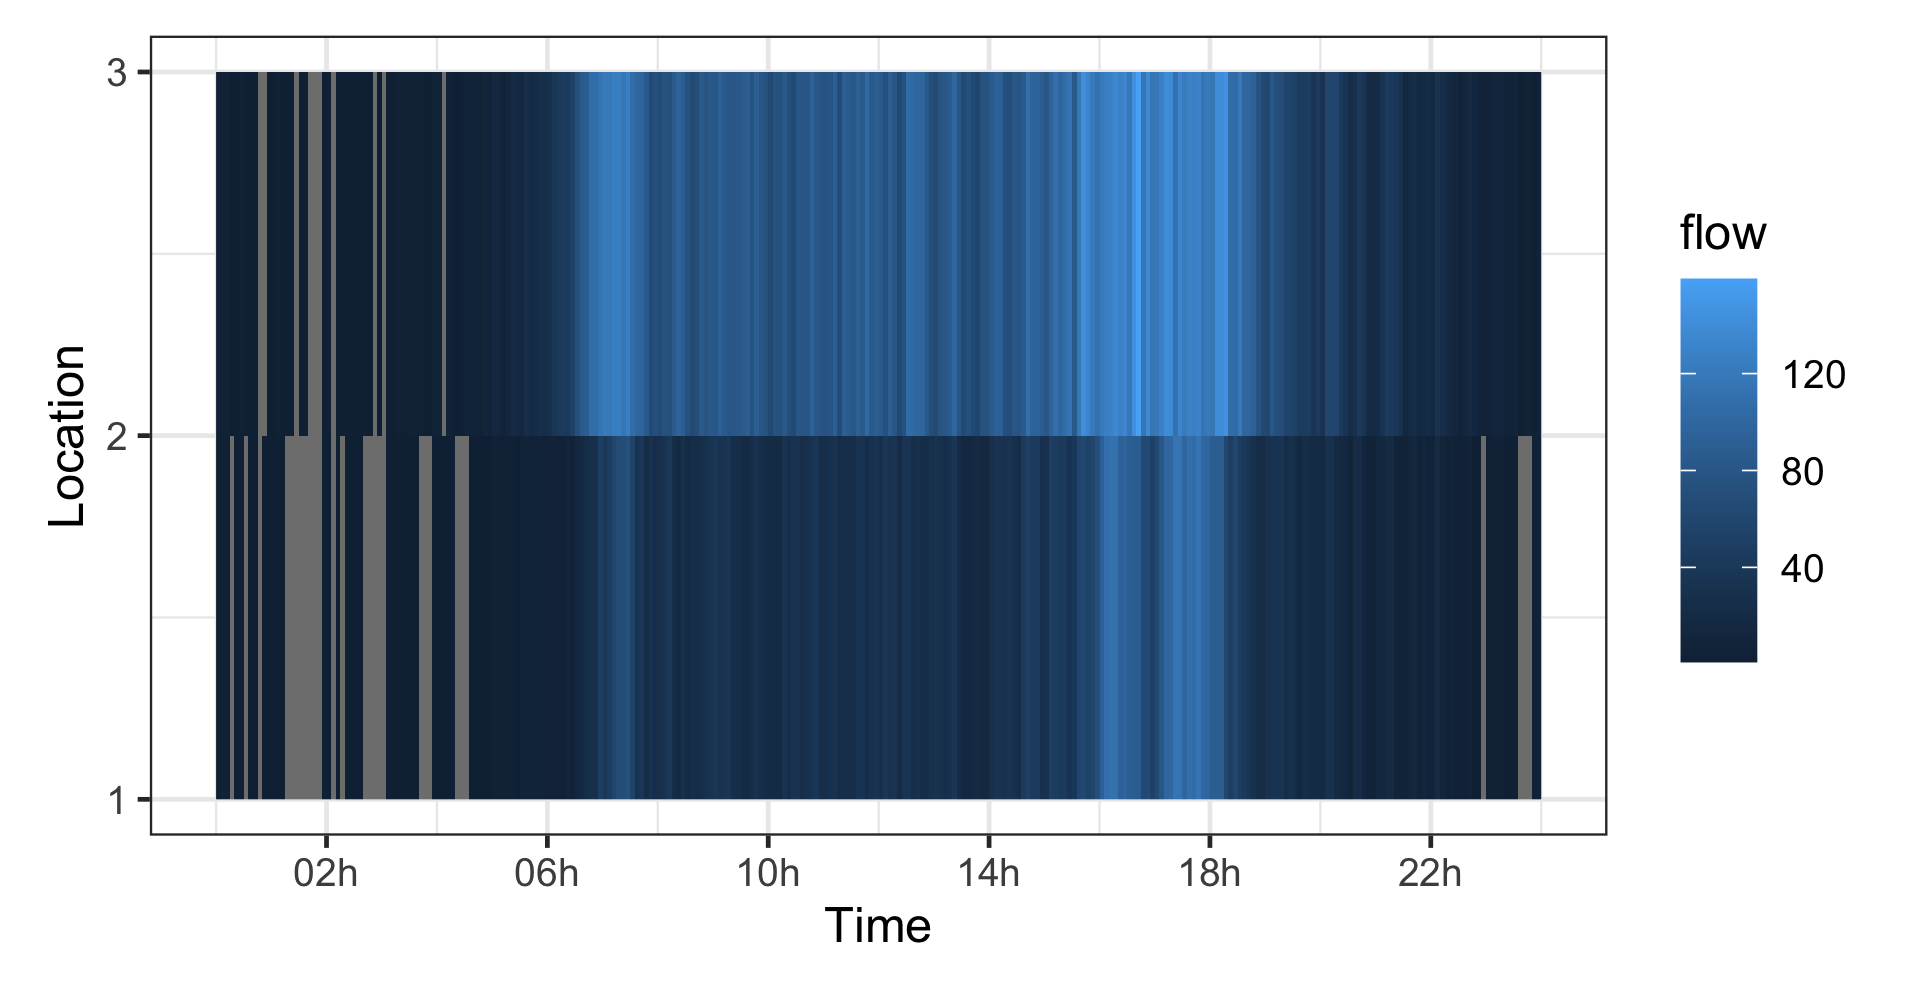
\includegraphics[width=0.50\linewidth]{MOTIVATING-EXAMPLE-1day-flow.png}}
      \subfloat{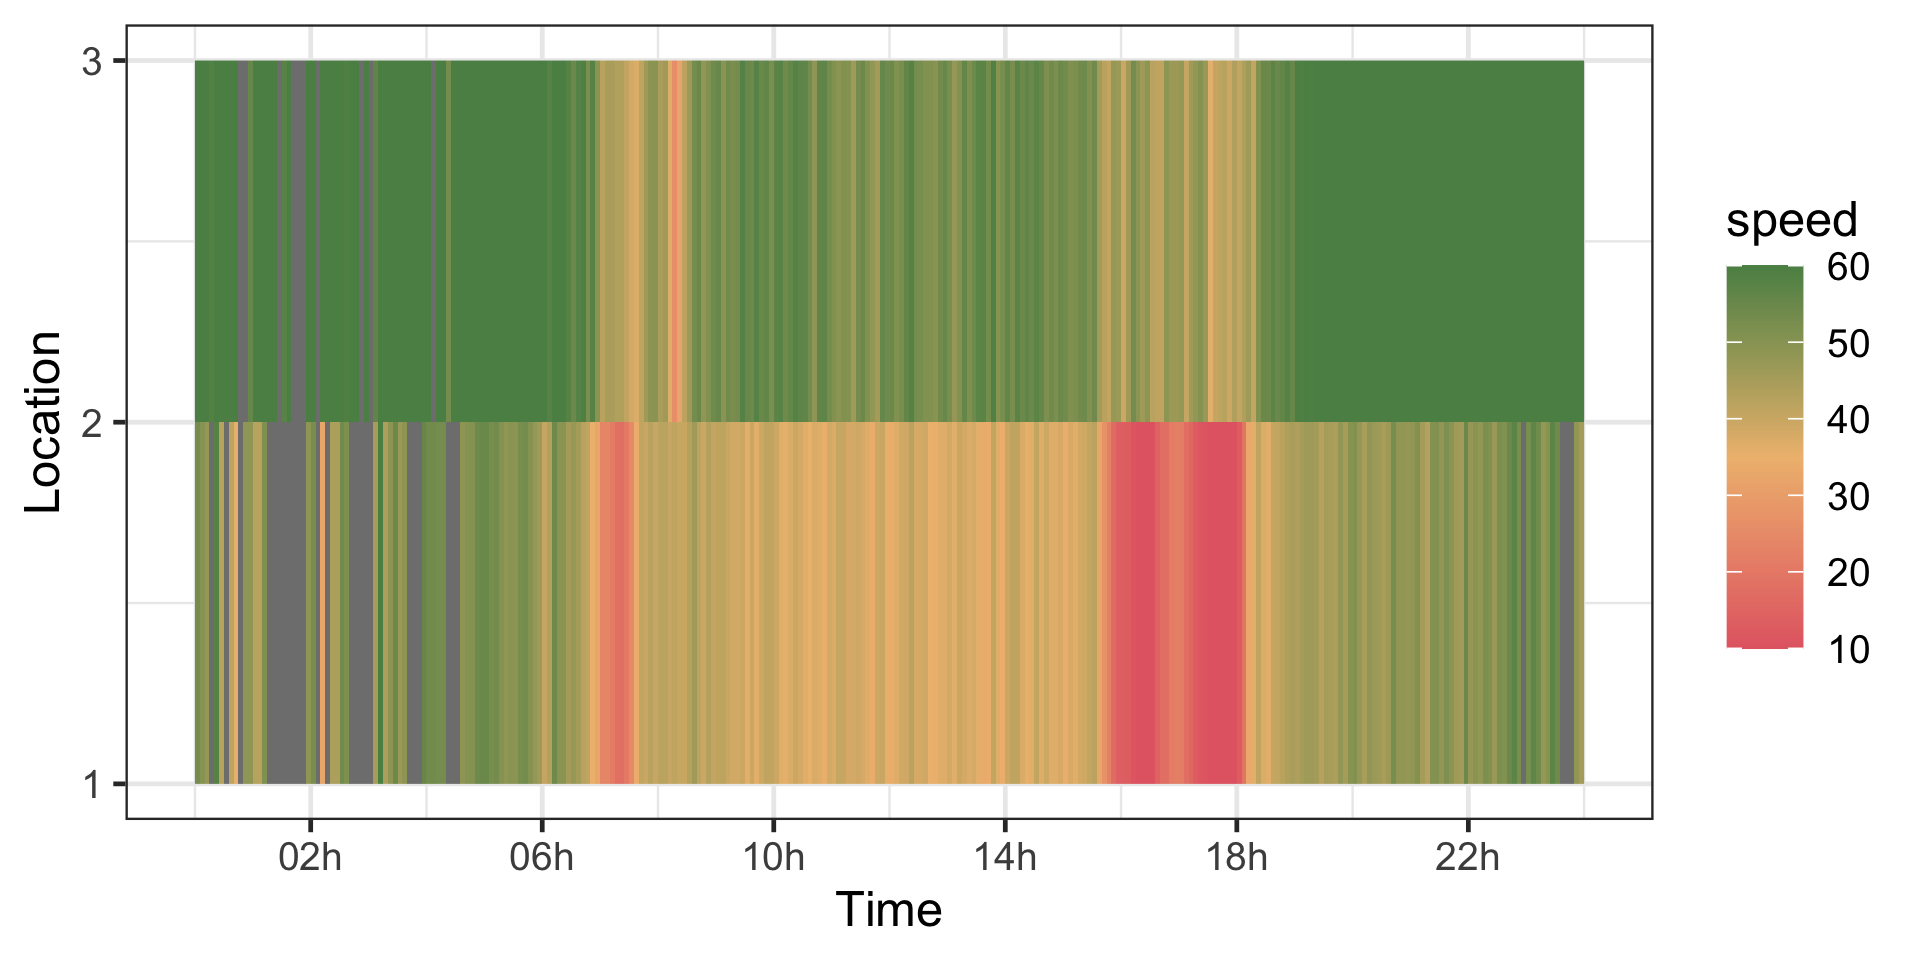
\includegraphics[width=0.50\linewidth]{MOTIVATING-EXAMPLE-1day-speed.png}}
      \caption{Speed and flow volume space-time plots for upstream camera pair
               (1-2) and downstream camera pair (2-3) on 5 Mar 2018.}
      \label{fig:motivating_example_1dayplots}
    \end{figure}

    % We do this by building a statistical model of traffic state.

    \heading{Activation model}

    We design our approach based on the model for freeway bottlenecks specified
    in \cite{chen2004}.
    Let $C = \{ s_j \}_{j=1}^{n}$ denote a road corridor monitored by a series
    of ANPR cameras placed along its path, where $s_j$ designates the $j$th
    segment (camera-pair) of the corridor. The sensors generate
    observations of traffic speed and flow, represented by $v(s_j, t)$ and
    $q(s_j, t)$ respectively, at each segment $j$ and time interval $t$. We are
    interested in whether the segments of $C$ are operating under localised
    congestion, particularly under the effect of a bottleneck. Let $A(s_j,t)$
    be a binary variable which indicates the presence of an active bottleneck in
    segment $j$ during time period $t$. We specify $A=1$ if the following
    inequalities are met:

    \begin{align}
    v(s_j, t) &< \theta \cdot v_f(s_j) \label{eq:active1} \\[10pt]
    \frac{v(s_{j+1}, t)}{v(s_j, t)} &> \frac{v_f(s_{j+1})}{v_f(s_j)} + \phi \label{eq:active2} \\[10pt]
    q(s_j, t) &> q_m(s_j) \label{eq:active3}
    \end{align}

    where $v_f(s_j)$ denotes the segment expected value of free flow speed;
     $q_m(s_j)$ indicates the typical-day median flow; $\theta$ is the
    upstream congestion factor; and $\phi$ is the factor that determines a
    substantial downstream speed gain.

    Criterion \ref{eq:active1} represents the presence of congestion upstream
    of the bottleneck; expression \ref{eq:active2} symbolises improved traffic
    flow downstream, operating in or close to free flow; and condition
    \ref{eq:active3} suggests user demand is within medium to high levels.
    We can not determine, however, the exact location of the bottleneck and
    where traffic breaksdown (we may be possibly able to infer it in some cases).

  \end{block}

\end{column}

\separatorcolumn

\begin{column}{\colwidth}

  \heading{Identification results}

  \begin{figure}[b]
    \centering
    \subfloat{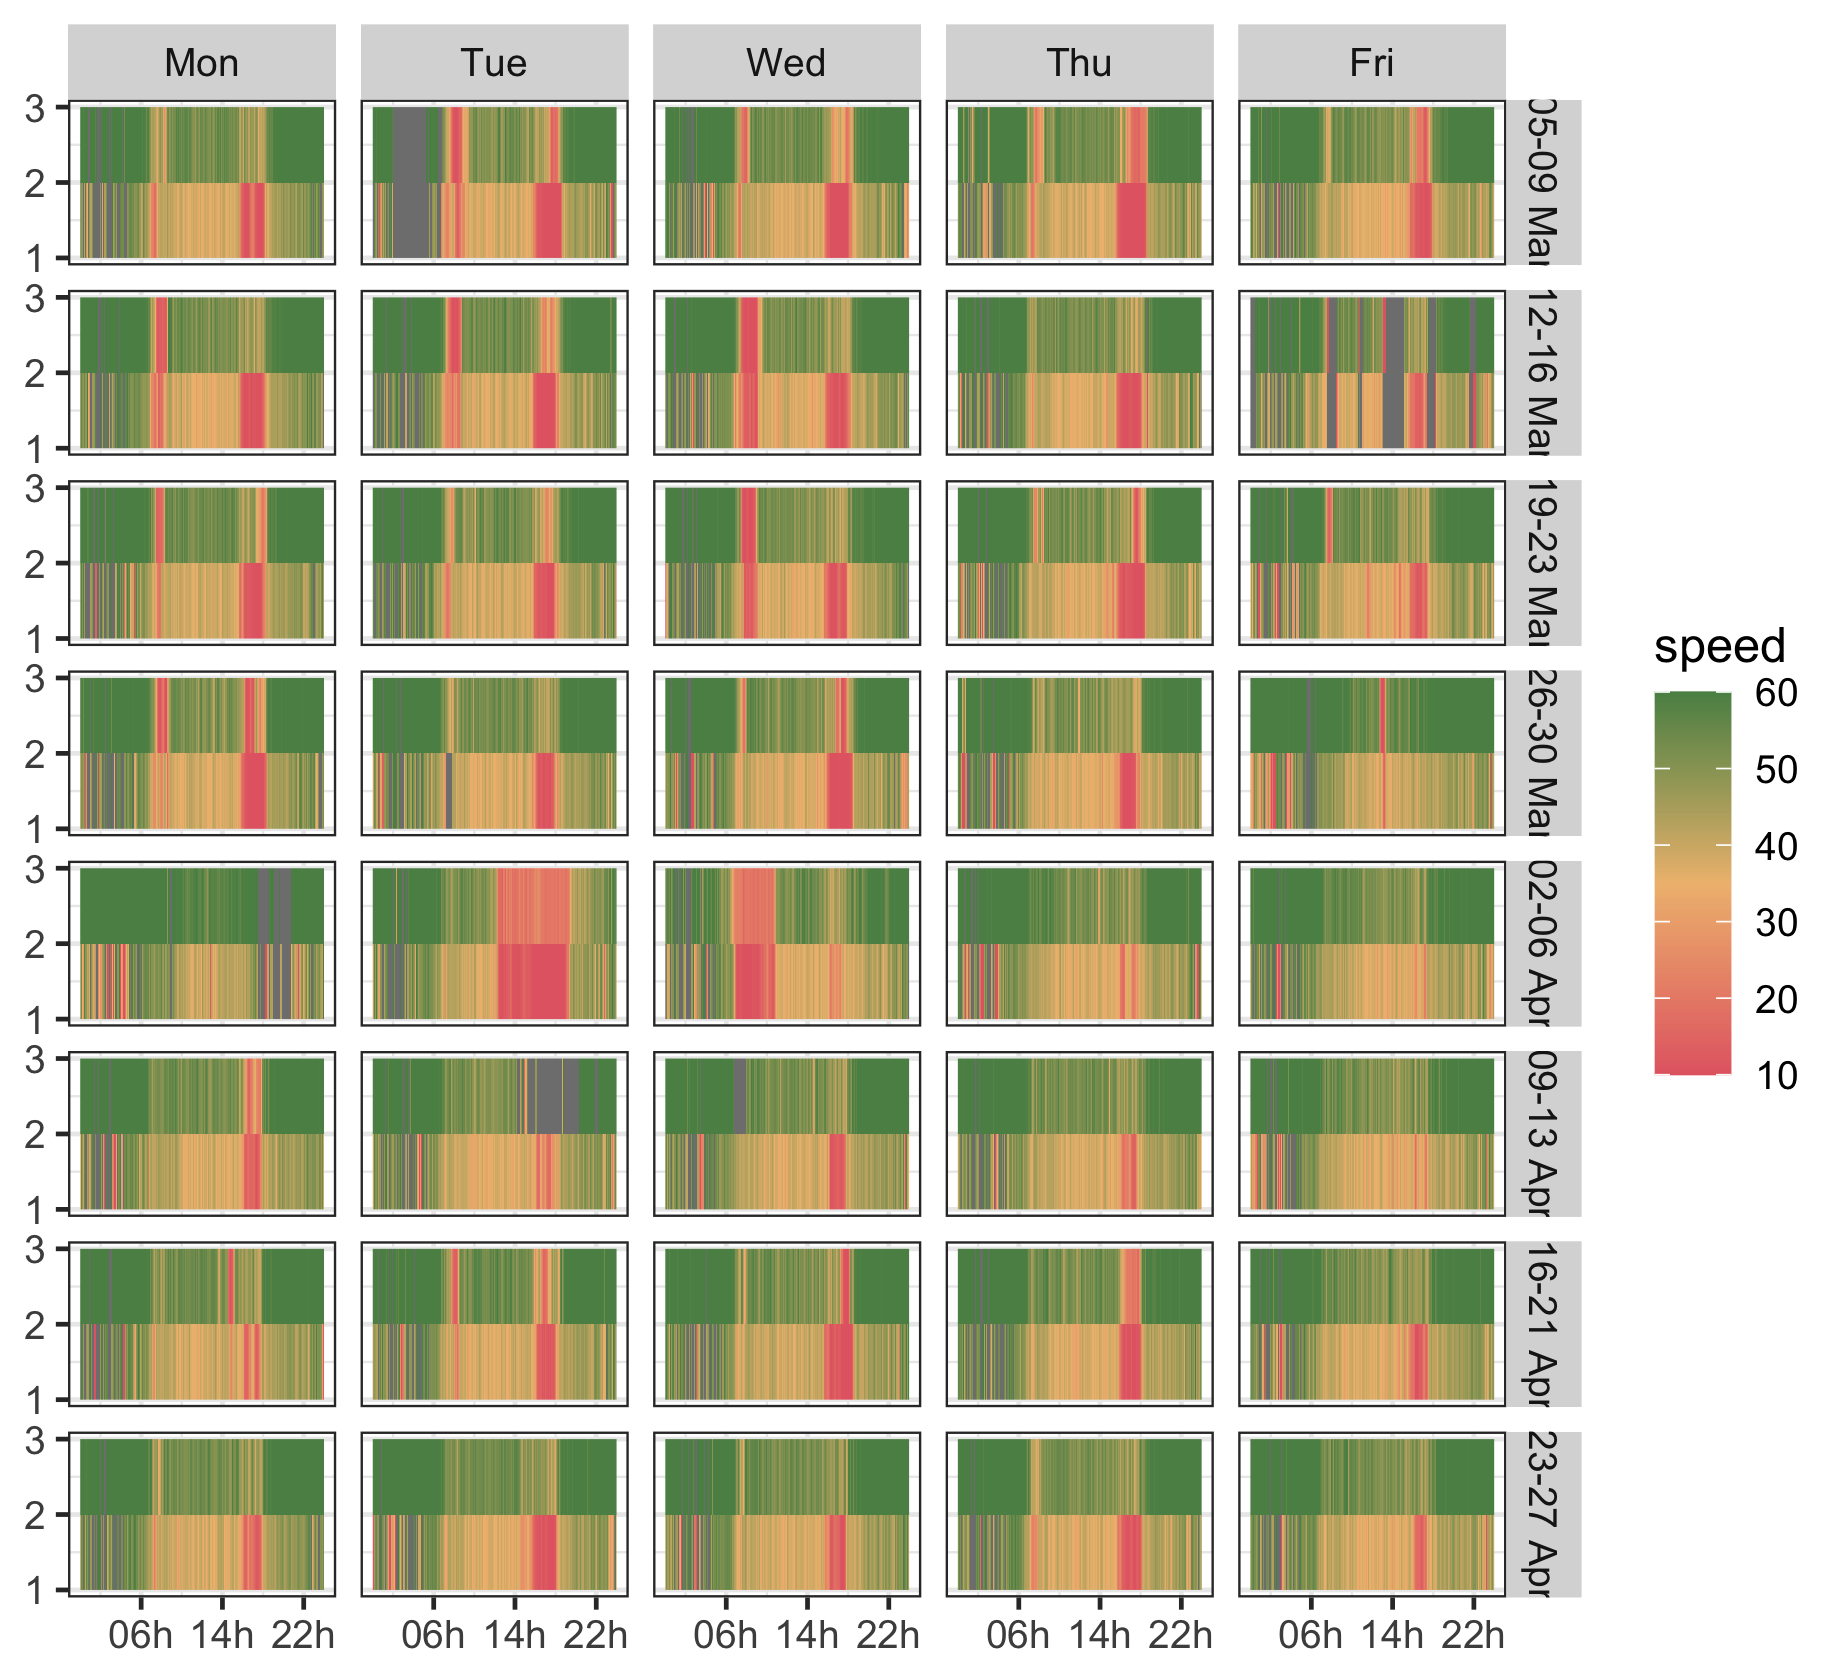
\includegraphics[width=0.50\linewidth]{MOTIVATING-EXAMPLE-8weeks-speed-shorter.png}}
    \subfloat{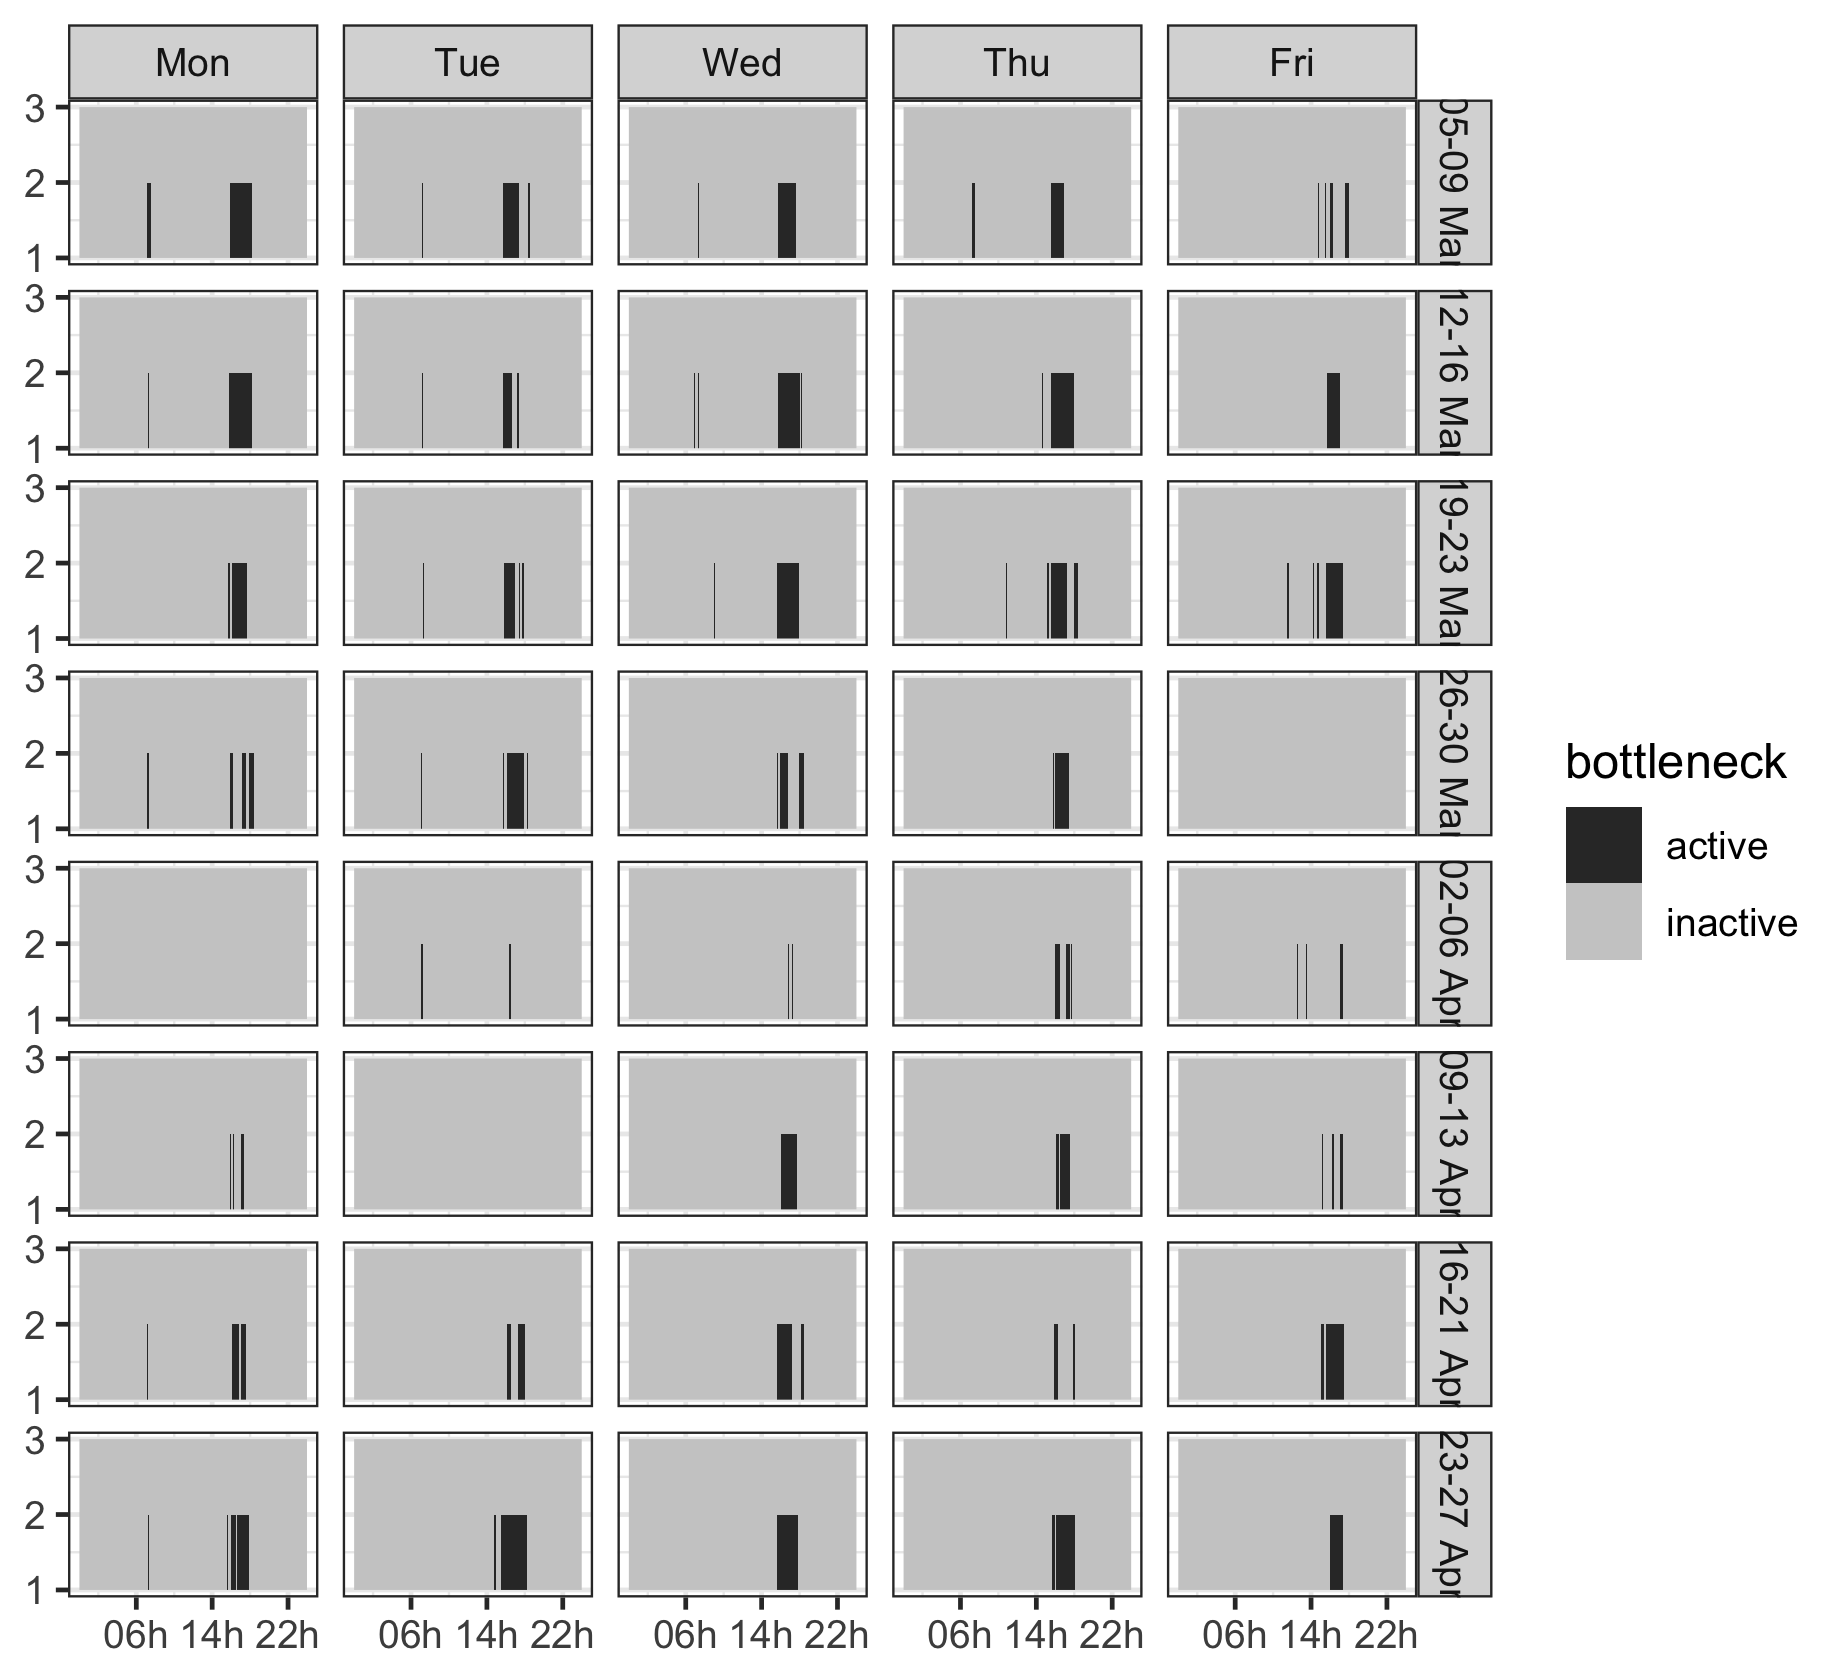
\includegraphics[width=0.50\linewidth]{MOTIVATING-EXAMPLE-8weeks-bottleneck-shorter.png}}
    \caption{Speed and bottleneck activation space-time plots for every weekday
             during a 8-week period in 2018.}
    \label{fig:motivating_example_8weeksplots}
  \end{figure}

  \begin{block}{Scaling bottleneck identification to the whole network}

      \heading{The corridor labelling problem}

      Since to,
      In order to run our identification algorithm across the whole network

      The corridor labelling

      - A flow graph is by itself not sufficient to


  \end{block}

  \begin{block}{References}

    \footnotesize{\bibliographystyle{abbrv}\bibliography{poster}}

  \end{block}

  \begin{columns}[c] % align columns

    \begin{column}{0.50\colwidth}

      \begin{figure}
        
\includegraphics[width=0.40\linewidth]{sponsor-bwhighres.jpg}
        \label{fig:epsrc_logo}
      \end{figure}

      \begin{figure}
        
\includegraphics[width=0.90\linewidth]{CDT_CCBD2.jpg}
        \label{fig:cdt_logo}
      \end{figure}

    \end{column}%

    \begin{column}{.50\colwidth}

      \begin{alertblock}{Contact}

        \begin{columns}[t] % align columns
          \begin{column}{0.25\colwidth}

            \begin{figure}
              \centering
              
\includegraphics[width=0.2\linewidth]{mail.png}
              \label{fig:mail}
            \end{figure}

            \centering\textbf{p.pinto-da-silva2@ncl.ac.uk}

          \end{column}%

          \begin{column}{0.25\colwidth}

            \begin{figure}
              \centering
              
\includegraphics[width=0.2\linewidth]{github.png}
              \label{fig:github}
            \end{figure}

            \centering\textbf{ppintosilva}

          \end{column}%

        \end{columns}

      \end{alertblock}

    \end{column}%
  \end{columns}


\end{column}

\separatorcolumn
\end{columns}
\end{frame}

\end{document}
